\documentclass[10pt,a4paper]{article}
\usepackage[utf8x]{inputenc}
\usepackage{ucs}
\usepackage{amsmath}
\usepackage{amsfonts}
\usepackage{amssymb}
\usepackage{hyperref}
\usepackage{graphicx}
\usepackage{float}
\usepackage{listings}

\usepackage[german]{babel}
\usepackage[T1]{fontenc}
%\usepackage[latin1]{inputenc}

% \lstset{language=bash,basicstyle=\footnotesize}%, numbers=left}
\lstset{language=bash, title=[CODEAUSSCHNITT], numbers=left, basicstyle=\footnotesize}

\author{Olaf Radicke}
\title{Dokumentation der Funktionsweise der OSR-Dracut-Module}


\begin{document}

\maketitle

\newpage 

\tableofcontents

\newpage 

\section{Gernerell}

Als erstes wird vom Kernel nach dem Booten ein kleiner Binär-Code von Dracut ausgeführt, der dann seinerseits die in dash geschriebene Dracut-Module ausführt. Das erste Modul das von Darcut startet wird ist das Modul 99base. Das Erste was das Modul tut ist, dafür zu sorgen das dass initramfs geladen hat. Das Script was dafür verantwortlich ist, ist die \texttt{init}-Datei. Diese kann angepasst werden. Empfohlen wird aber stat dessen die Hooks zu verwenden. Hooks sind Scrips die vor oder nach definierten Ereignissen ausgeführt werden. Diese Hooks werden in den Modulen in den Dateien \texttt{install} definiert.

Die Hooks die Dracut abarbeitet stehen im initrd im Verzeichnis \texttt{/lib/dracut/hooks/}. Die Einträge werden von Dracut automatisch generiert.

\subsection{Verwendete Hooks}

Die in den Modulen verwendeten Hooks sind:
\begin{description}
 \item[cmdline] Ein sehr früher Zeitpunkt. Hier werden die Kerne-Parameter ausgewertet werden die dem Bootloader mitgegeben wurden (Sei es als GRUB-Konfiguration oder beim Booten). Hier werden z.B. die wichtigsten Environment-Variablen gesetzt. 
 \item[pre-pivot] Das ist der letzte Hook der ausgeführt wird, bevor  das richtige root-Verzeichnis ein gehangen wird. Also ein guter Zeitpunkt für etweilige Aufräumarbeiten.
\end{description}
 
\subsection{Verwendete undokumentierte Hooks}

Die volgenen Hooks ist in der Dracut-Doku nicht dokumentiert. Werden aber verwendet.

\begin{description}
 \item[emergency] wenn der Bootvorgang wegen einer Ausnahme unterbrochen werden muss, wird der Hook aufgeruffen.
 \item[netroot] Scheint es nicht (mehr) zu geben.
\end{description}

In einem Script \texttt{check} wird eine Funktion \texttt{check()} definiert. Das Scrip \texttt{check} sollte 0 (null) zurückgeben, wenn alle Bedingungen erfüllt sind. Wird ein anderer Wert zurückgegeben, wird das Modul nicht von Darcut geladen.

\subsection{Weitere Schlüsselworte (Methoden) von Dracut}

\begin{description}
 \item[inst\_simple] Mit dem Schlüsselwort \texttt{inst\_simple} werden Dateien in das initramfs kopiert/installiert.
 \item[dracut\_install] Mit dem Schlüsselwort \texttt{dracut\_install} werden Software-Pakete in die ramsf-Umgebung installiert bzw. zur Verfügung gestellt.
 \end{description}
 
\subsection{Verwendete Darcut-Lib-Komandos}

Die Dracut-lib (\texttt{/usr/share/dracut/modules.d/99base/dracut-lib.sh}) stellt verschiedene Methoden zur Verfühgung. Benutzt werden von OSR:

\begin{description}
 \item [getarg()] Gibt die benutzten Kernel-Parameter zurück.
 \item [die()] Schreibt eine Meldung in \texttt{/dev/kmsg}, gibt eine Meldung auf der Standartausgabe aus und beendet das Script mit Rückgabelwert 1.
 \item [info()] Schreibt Meldungen in  \texttt{/dev/kmsg}, mit die Informationen später, nach dem Booten vom Benutzer abgerufen werden können.

\end{description}


\subsection{Der Bootablauf für com.oonics}


\begin{itemize}
 \item Basic Setup
    \begin{itemize}
      \item Nichts für com.oonics
    \end{itemize}
 \item Hook "`\textbf{cmdline}"'
    \begin{description}
      \item [1 - setup-osrenv.sh] (Modul: osr) Ermittlung der Distrebution.
      \item [2 - parse-nodeid.sh] (Modul: osr] Überprüft noch mal die
      Distrebution und ermitteld die Node-ID.
      \item [10 - parse-root-opts.sh] (Modul: base) Base-Modul von Dracut
      schreibt in die Datei: \texttt{/tmp/root.info}
      \item [90 - parse-nfsroot.sh] (Modul: nfs) Der Hook des Dracut-Modul für
      nfs-root wird aufgerufen.
      \item [99 - parse-cdsl.sh] (Modul: osr) Es wird eine Datenbank mit den
      Informationen zu cdsl angelegt.
    \end{description}
 \item Hook "`\textbf{pre-udev}"'
    \begin{description}
      \item [59 - osr-net-genrules.sh (Modul: osr-cluster)] Es werden
      udev-Regeln gesetzt.
    \end{description}
 \item Start Udev
    \begin{itemize}
      \item Nichts für com.oonics
    \end{itemize}
 \item Hook "`\textbf{pre-trigger}"'
    \begin{itemize}
      \item Nichts für com.oonics
    \end{itemize}
 \item Trigger Udev
    \begin{itemize}
      \item Nichts für com.oonics
    \end{itemize}
 \item Main Loop
    \begin{itemize}
      \item Nichts für com.oonics
    \end{itemize}
 \item Hook "`\textbf{pre-mount}"'
    \begin{description}
      \item [11 - osr-detect-chroot.sh] (Modul: osr-chroot) Wenn eine Node-ID
      gefunden wird, werden die Node-Informationen geladen. Es wird geprüft ob
      eine chroot-Umgebung benötigt wird.
    \end{description}
 \item Hook "`\textbf{mount}"'
    \begin{itemize}
      \item Nichts für com.oonics
    \end{itemize}
 \item Hook "`\textbf{pre-pivot}"'
    \begin{description}
      \item [12 - osr-mount-chroot.sh] (Modul: osr-chroot) Es wird versuch das
      sharedroot zu mounten.
      \item [51 - osr-move-chroot.sh] (Modul: osr-chroot) Wechsel (chroot) in
      das sharedroot.
      \item [90 - write-xfiles.sh] (Modul: osr) Abhängig von Filesystem, wird
      eine andere Lib gewählt, eine \texttt{/etc/xtab}, eine  \texttt{xrootfs}
      und eine \texttt{xkillall\_procs} erstellt.
      xkillall-Prozess gestartet.
      \item [60 - mount-cdsl.sh] (Modul: osr) bind-mount für das Chared-Root-File-System
      \item [99 - nfsroot-cleanup.sh] (Modul: nfs) cleanup-Przess für NFS.
    \end{description}
 \item Hook "`\textbf{cleanup and switch\_root}"'
\end{itemize}



\subsection{Undokumentierte Dracut-Schnittstellen}


An dieser Stelle wird das root-Filesystem präperiert (\textbf{/modules.d/95osr-cluster/osr-detect-root.sh} ):


\begin{lstlisting}
if [ -z "$oldroot" ] || [ "$oldroot" = "autodetect" ]; then
    info "[osr-detect-root]: fstype: ${fstype} root: ${root} netroot: $netroot"
    # Network root scripts may need updated root= options,
    # so deposit them where they can see them (udev purges the env)
    {
        echo "root='$root'"
        echo "rflags='$rflags'"
        echo "fstype='$fstype'"
        echo "netroot='$netroot'"
        echo "NEWROOT='$NEWROOT'"
    } > /tmp/root.info
\end{lstlisting}

\bigskip
In der Datei \textbf{95osr-cluster/module-setup.sh} wird der Filesystem-Typ-Handler gesetzt. Dername setzt sich zusammen aus [fs-typ] und "root":

\bigskip

\begin{lstlisting}
    # set fstyp-handler
    echo '[ -e $NEWROOT/proc ]' > $hookdir/initqueue/finished/osrroot.sh

    # Handler
    inst_simple "$moddir/osr-detect-root.sh" "/sbin/osrroot"
\end{lstlisting}


\bigskip

Handler für den netroot-Typ ( \texttt{/usr/share/dracut/modules.d/40network/netroot} ):

\bigskip

\begin{lstlisting}
# Check: do we really know how to handle (net)root?
[ -z "$root" ] && die "No or empty root= argument"
[ -z "$rootok" ] && die "Don't know how to handle 'root=$root'"

handler=${netroot%%:*}
handler=${handler%%4}
handler="/sbin/${handler}root"
if [ -z "$netroot" ] || [ ! -e "$handler" ] ; then
    die "No handler for netroot type '$netroot'"
fi
\end{lstlisting}

\bigskip

Bzw.: \texttt{/modules.d/95osr-cluster/install}

\bigskip

\begin{lstlisting}
inst "$moddir/osr-detect-root.sh" "/sbin/osr-detect-root"
inst "$moddir/osr-detect-root.sh" "/sbin/osrroot"
\end{lstlisting}

%%%%%%%%%%%%%%%%%%%%%%%%%%%%%%%%%%%%%%%%%%%%%%%%%%%%%%%%%%%%%%%%%%%%%%%%%%%%%%%%
% Die einzelen Module....
%%%%%%%%%%%%%%%%%%%%%%%%%%%%%%%%%%%%%%%%%%%%%%%%%%%%%%%%%%%%%%%%%%%%%%%%%%%%%%%%


%%%%%%%%%%%%%%%%%%%%%%%%%%%%%%%%% NEW SECTION %%%%%%%%%%%%%%%%%%%%%%%%%%%%%%%%%%
\section{Modul 95osr-chroot}

\subsection{Definierte Hooks}

\begin{tabular}{|l|l|l|}
 \hline
\textbf{Hook} & \textbf{Priorität} & \textbf{Script} \\ \hline
netroot  & 11 & osr-detect-chroot.sh \\ \hline
netroot  & 50 & osr-mount-chroot.sh \\ \hline
pre-udev & 51 & osr-move-chroot.sh \\ \hline
\end{tabular}

\subsubsection{osr-detect-chroot.sh}

Siehe \ref{osrdetectchroot} Seite \pageref{osrdetectchroot}.

\subsubsection{osr-mount-chroot.sh}

Siehe: \ref{osrmountchroot} Seite \pageref{osrmountchroot}.

\subsubsection{osr-move-chroot.sh}

\begin{description}
\item[Hook:] pre-pivot
\item[Priorität:] 51
\end{description}

Das Modul wechselt in das sharedroot.

%%%%%%%%%%%%%%%%%%%%%%%%%%%%%%%%% NEW SECTION %%%%%%%%%%%%%%%%%%%%%%%%%%%%%%%%%%

\section{Modul 95osr-cluster}

\subsection{Von Dracut zu installierende Software}

\begin{itemize}
 \item tr
 \item expr
 \item mkdir
 \item basename
\end{itemize}

\subsection{Definierte Hooks}

\begin{tabular}{|l|l|l|}
 \hline
\textbf{Hook} & \textbf{Priorität} & \textbf{Script} \\ \hline
pre-udev   & 59 & osr-net-genrules.sh \\ \hline
netroot    & 11 & osr-detect-chroot.sh \\ \hline
netroot    & 50 & osr-mount-chroot.sh \\ \hline
\end{tabular} 


\subsubsection{osr-net-genrules.sh}

\begin{description}
\item[Hook:] pre-udev
\item[Priorität:] 59
\end{description}

Das Script setzt die udev-Regeln.

\subsubsection{osr-detect-chroot.sh}
\label{osrdetectchroot} 

\begin{description}
\item[Hook:] netroot
\item[Priorität:] 11
\end{description}

Das Script überprüft, ob für den Node eine ID gesetzt ist. Wenn nicht bricht es mit einer Fehlermeldung ab. Ist die ID gesetzt wird \verb|/etc/conf.d/osr-nodeidvalues-${nodeid}.conf| eingebunden. Dann wird geprüft ob eine chroot-Umgebung gebraucht wird. Das Ergebnis der Prüfung wird gespeicherte mit \texttt{osr\_param\_store()}

\begin{figure}[H]
 \centering
 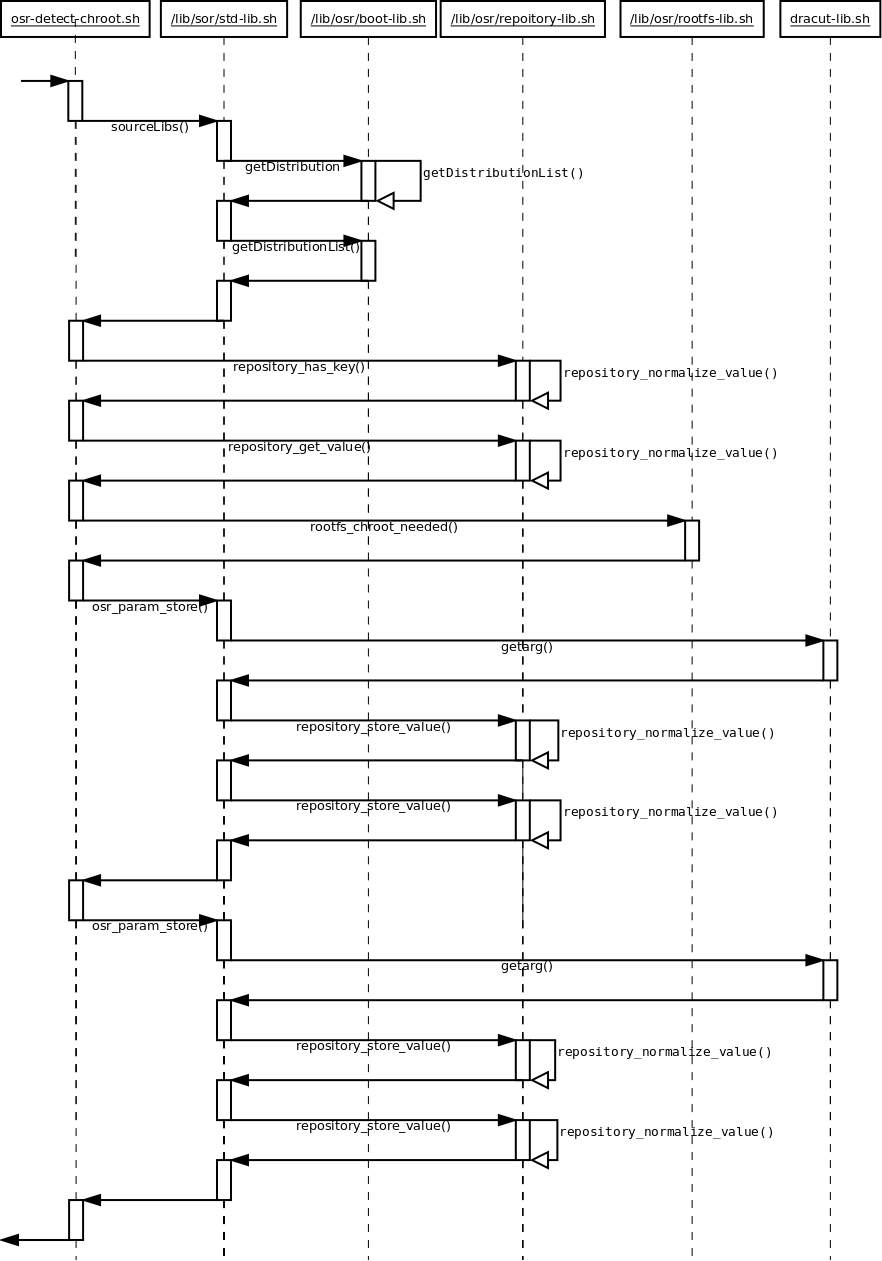
\includegraphics[width=1.0\textwidth,height=1.0\textwidth]{./sequence_diagram_osr-detect-chroot_DE_de.png}
 \caption[]{Sequence-Diagram des osr-detect-chroot.sh-Scrips}
\end{figure}

\subsubsection{osr-mount-chroot.sh}
\label{osrmountchroot} 

\begin{description}
\item[Hook:] netroot
\item[Priorität:] 50
\end{description}

Das Script hängt das richtige (shared) root-Verzeichnis ein. Schlägt das fehl, wird versucht das noch ein mal mit default Werten zu versuchen. Dann Werden die nötigen Ordnerstrukturen kopiert und die besonderen Verzeichnisse eingehangen.

\begin{verbatim}
  cp -axf $chroot_source $chroot_path
  rm -rf $chroot_path/var/run/*
  mkdir -p $chroot_path/tmp
  chmod 755 $chroot_path
  mount -t tmpfs none $chroot_path/dev
  cp -a /dev $chroot_path/
  mount -t devpts none $chroot_path/dev/pts
  mount -t proc proc $chroot_path/proc
  mount -t sysfs sysfs $chroot_path/sys
\end{verbatim}

\begin{figure}[H]
 \centering
 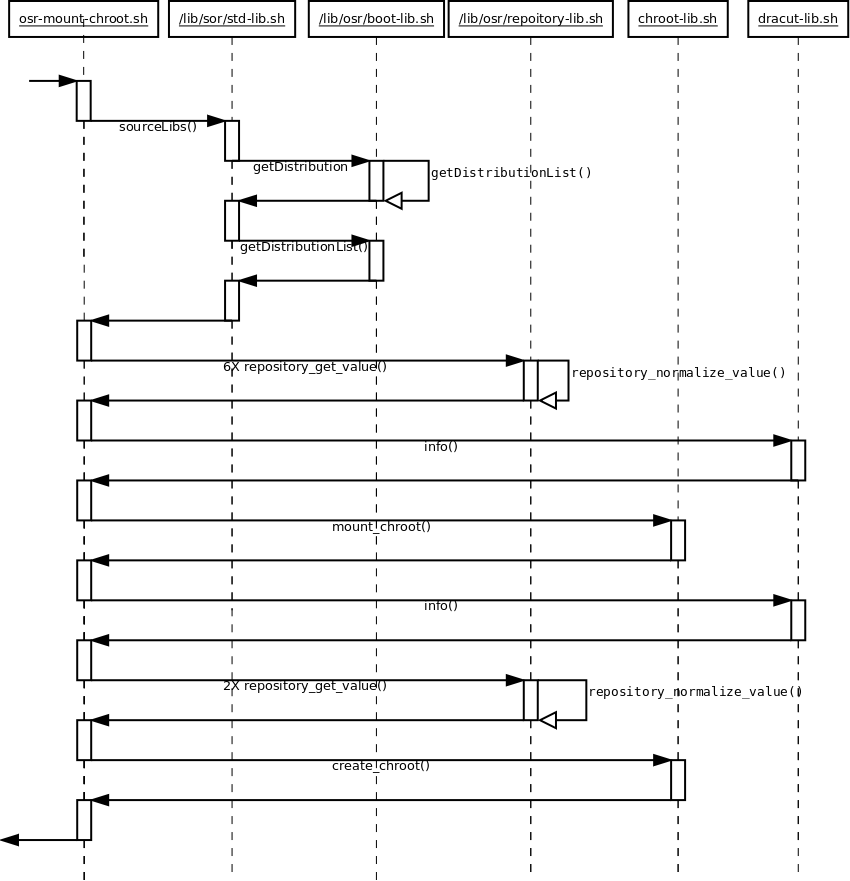
\includegraphics[width=1.0\textwidth,height=1.0\textwidth]{./sequence_diagram_osr-mount-chroot_DE_de.png}
 \caption[]{Sequence-Diagram des osr-mount-chroot.sh-Scrips}
\end{figure}


%%%%%%%%%%%%%%%%%%%%%%%%%%%%%%%%% NEW SECTION %%%%%%%%%%%%%%%%%%%%%%%%%%%%%%%%%%

\section{Modul 96osr}

Das Modul ist dafür zuständig, das File System für ein \texttt{shared root} ein zu hängen.

\subsection{In Initramfs installierte Dateien}

\begin{itemize}
 \item \verb|<|moddir\verb|>| /issue nach /etc
 \item \verb|<|moddir\verb|>|/shinit.sh nach /sbin
 \item \verb|<|moddir\verb|>|/lib/boot-lib.sh nach /lib/osr
 \item \verb|<|moddir\verb|>|/lib/defaults.sh nach /lib/osr
 \item \verb|<|moddir\verb|>|/lib/repository-lib.sh nach /lib/osr
 \item \verb|<|moddir\verb|>|/lib/rootfs-lib.sh nach /lib/osr
 \item \verb|<|moddir\verb|>|/lib/shinit.sh nach /lib/osr
 \item \verb|<|moddir\verb|>|/lib/std-lib.sh nach /lib/osr
\end{itemize}

\subsection{Von Dracut zu installierende Software}

\begin{itemize}
 \item awk
 \item cut
 \item tr
 \item expr
 \item mkdir
 \item basename
\end{itemize}

expr könnte mit awk abgedeckt werden.

\subsection{Definierte Hooks}

\begin{tabular}{|l|l|l|}
 \hline
\textbf{Hook} & \textbf{Priorität} & \textbf{Script} \\ \hline
setup-osrenv.sh  & 99 & cmdline \\ \hline
parse-nodeid.sh  & 2 & cmdline \\ \hline
parse-cdsl.sh & 99 & cmdline \\ \hline
mount-cdsl.sh & 1 & pre-pivot \\ \hline
write-xfiles.sh & 90 & pre-pivot \\ \hline
emergencyenv.sh & 1 & emergency \\ \hline
\end{tabular} 

\subsubsection{setup-osrenv.sh}
\begin{description}
\item[Hook:] cmdline
\item[Priorität:] 99
\end{description}

\begin{figure}[H]
 \centering
 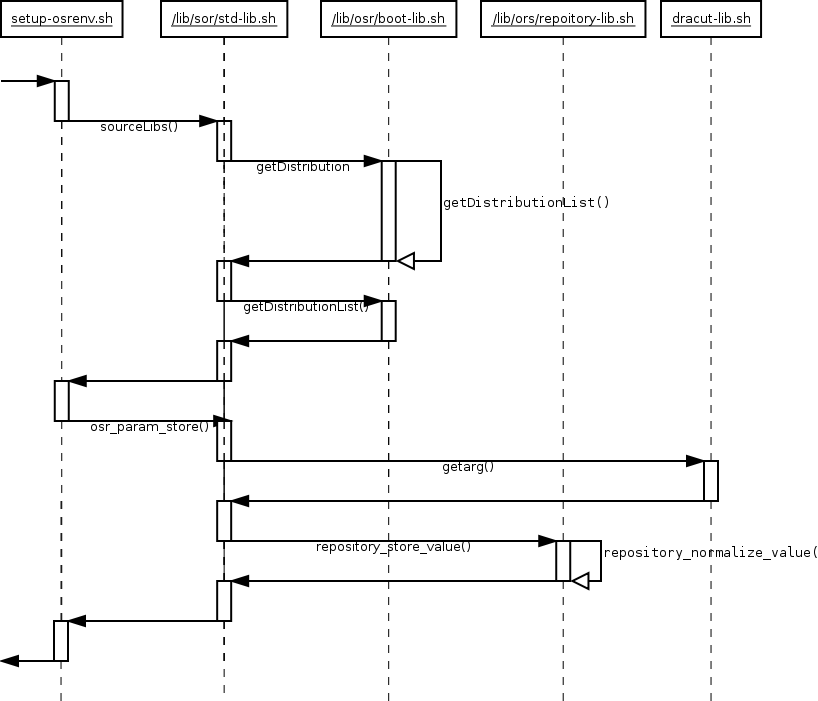
\includegraphics[width=1.0\textwidth,height=1.0\textwidth]{./sequence_diagram_setup-osrenv_DE_de.png}
 \caption[]{Sequence-Diagram des setup-osrenv.sh-Scrips}
\end{figure}

Das Script lädt \texttt{dracut-lib.sh} und die \texttt{/osr/std-lib.sh}. Das Script versucht herauszufinden um welche Distribution es sich handelt. Und legt dann eine einfache Datenbank  mit Schlüssel-Werte-Paaren an. Die Schlüssel der gespeicherte Werte sind:
\medskip 

\begin{tabular}{|l|l|}
 \hline
\textbf{Name} & \textbf{ Wert} \\ \hline
logofile          & \verb|"/etc/atix-logo.txt"|  \\ \hline
shellrcfile       & \verb|${libdir}/shinitrc|  \\ \hline
shellissue        & \verb|${predir}/etc/issue|  \\ \hline
shellissuetmp     & \verb|${predir}/tmp/issue|  \\ \hline
shell             & \verb|"/bin/bash --rcfile $(repository_get_value shellrcfile)"|  \\ \hline
sysctlfile        & \verb|"${predir}/etc/sysctl.conf"|  \\ \hline
xtabfile          & \verb|/etc/xtab|  \\ \hline
xrootfsfile       & \verb|/etc/xrootfs|  \\ \hline
xkillallprocsfile & \verb|/etc/xkillallprocs|  \\ \hline
\end{tabular} 


\subsubsection{parse-nodeid.sh}
\begin{description}
\item[Hook:] cmdline
\item[Priorität:] 2
\end{description}

\begin{figure}[H]
 \centering
 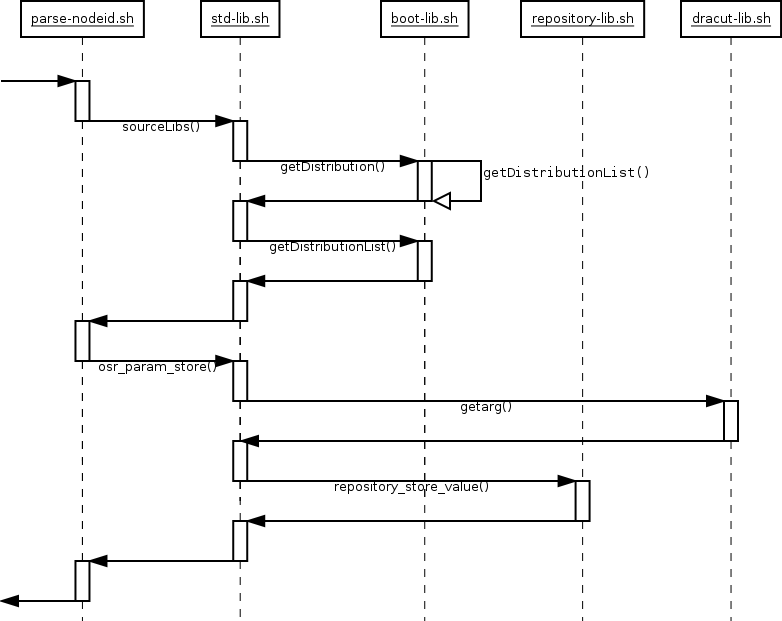
\includegraphics[width=1.0\textwidth,height=1.0\textwidth]{./sequence_diagram_parse-nodeid_DE_de.png}
 \caption[]{Sequence-Diagram des parse-nodeid.sh-Scrips}
\end{figure}

Das Script überprüft noch ein mal die Art der Distribution und speichert den Namen in eine einfache Schlüssel-Werte-Tabelle (mittels der Funktion \texttt{repository\_store\_value()} aus der Datei  \texttt{repository-lib.sh})
Das Script überprüft ob beim booten die Node-ID als Parameter übergeben wurde.


\subsubsection{parse-cdsl.sh}
\begin{description}
\item[Hook:] cmdline
\item[Priorität:] 99
\end{description}

Das Scrip legt in eine einfache Datenbank mit Schlüssel-Werte-Paaren an. Die Schlüssel der gespeicherte Werte sind:

\medskip 

\begin{tabular}{|l|l|}
 \hline
\textbf{Name} & \textbf{ Wert} \\ \hline
cdsltree & /cluster/cdsl \\ \hline
cdslsharedtree & /cluster/shared \\ \hline
cdsllink & /cdsl.local \\ \hline
\end{tabular} 

\subsubsection{mount-cdsl.sh}
\begin{description}
\item[Hook:] pre-pivot
\item[Priorität:] 1
\end{description}

Das Script macht den --bind-mount für das Chared-Root-File-System. Das wird mit cdsllinks realisiert.

\begin{figure}[H]
 \centering
 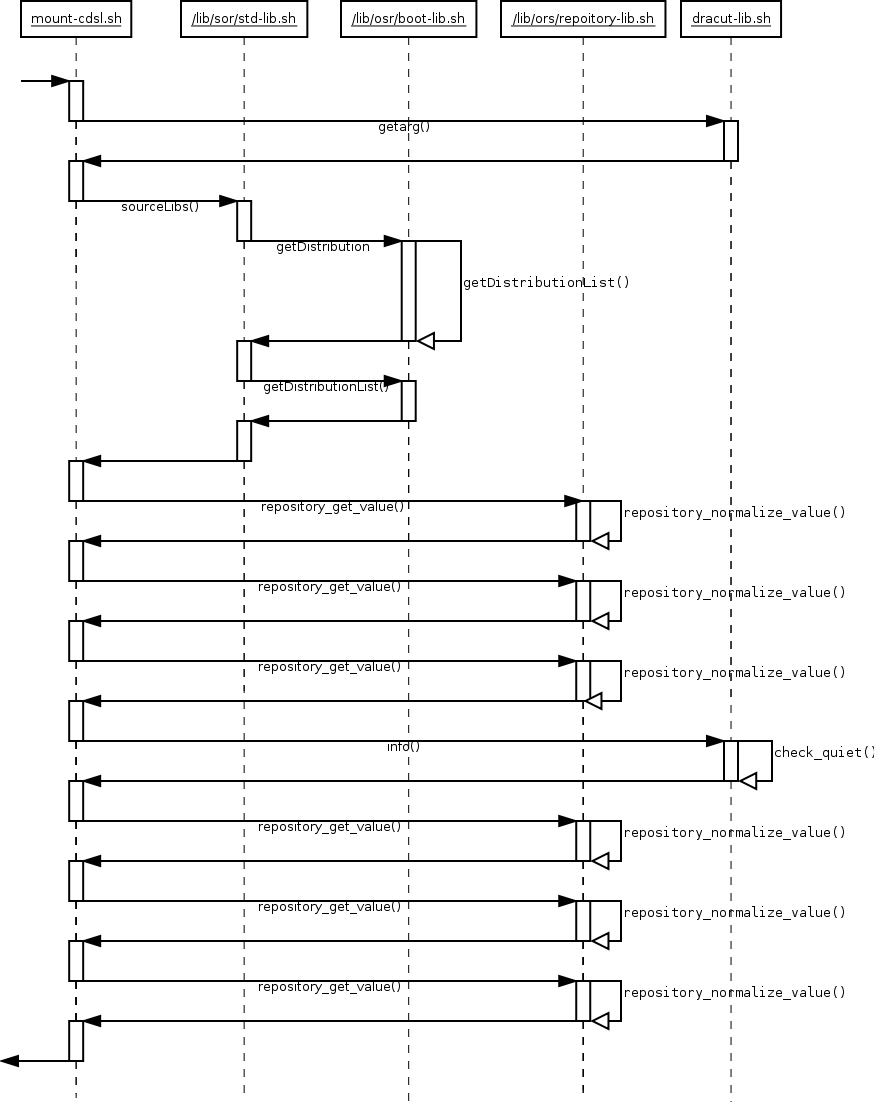
\includegraphics[width=1.0\textwidth,height=1.0\textwidth]{./sequence_diagram_mount-cdsl_DE_de.png}
 \caption[]{Sequence-Diagram des mount-cdsl.sh-Script}
\end{figure}


\subsubsection{write-xfiles.sh}
\begin{description}
\item[Hook:] pre-pivot
\item[Priorität:] 90
\end{description}

Je nach verwendeten File-System des Chared-Root-Tree wird eine bestimmte Lib eingehangen. Dann die /etc/xtab erstellt bzw.  generiert. Dann wird das \texttt{xrootfs} erstellt und der \texttt{xkillall\_procs}.

\begin{figure}[H]
 \centering
 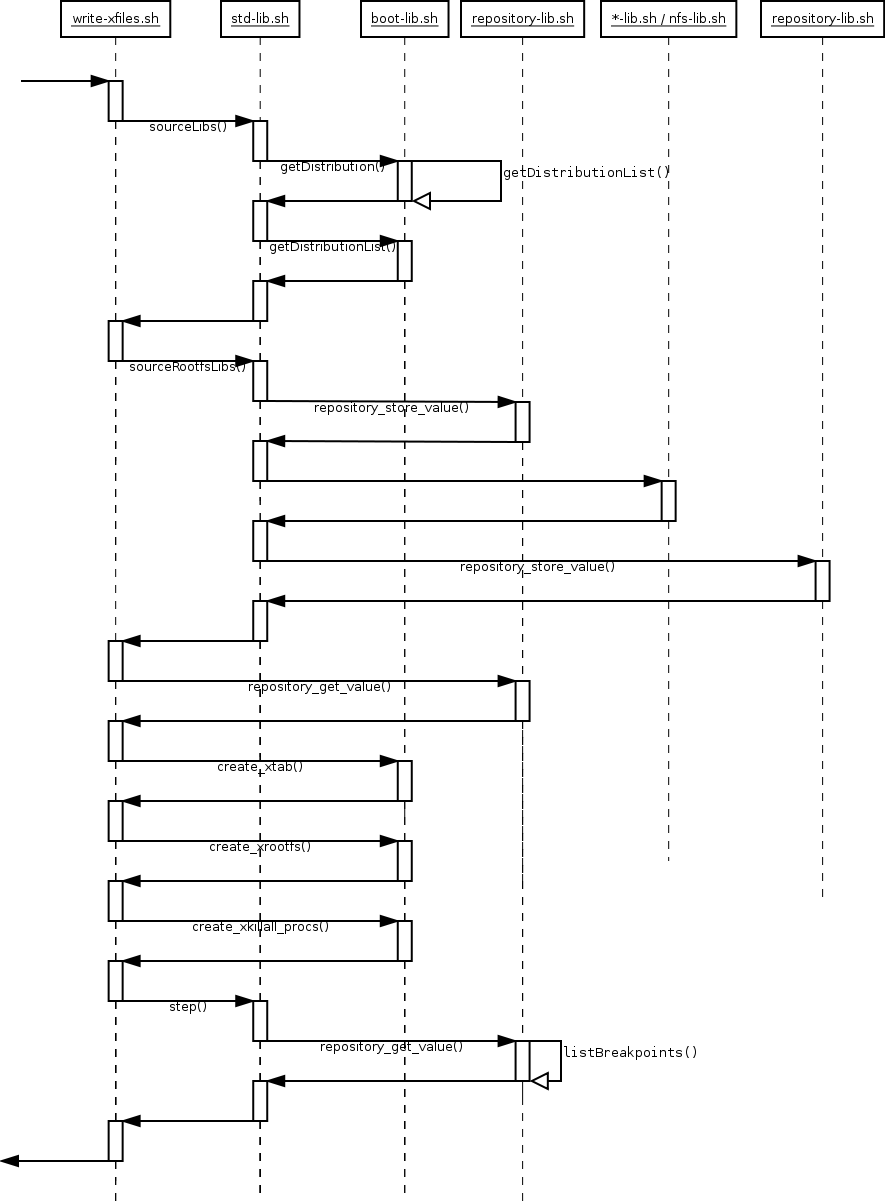
\includegraphics[width=1.0\textwidth,height=1.0\textwidth]{./sequence_diagram_write-xfiles_DE_de.png}
 \caption[]{Sequence-Diagram des write-xfiles.sh-Script}
\end{figure}

\subsubsection{emergencyenv.sh}
\begin{description}
\item[Hook:] emergency
\item[Priorität:] 1
\end{description}

Das Script sorgt für ein Semigraphische Login-Graphik. Dies geschieht durch das setzen der ENV-Variable auf das Script /sbin/shinit.sh.

\section{Modul 99osr-atix-legacy}

Das Modul stellt lediglich ein Semigrafisches Logo zur Verfügung, was dem User beim Login gezeigt wird.

\section{Coding conventions}

\subsection{AWK}

\subsubsection{Vorteile von AWK}

AWK bietet eine ganze Reihe von Vorteilteilen gegenüber Dash/Bash.

\begin{itemize}
 \item Es ist keine Entweder-oder-Entscheidung. Dash/Bash und lässt sich relativ gut wischen.
 \item AWK kommt von der Syntax C sehr nahe. Da die meisten Sprachen auf C-Syntax
       basieren (Perl, C++, Java, C\#, JavaScript, PHP...), dürfe es leichter sein,
       (neue) Programmiere für das Projekt zu gewinnen.
 \item AWK hat mit den Flag \verb|-W lint|  ein mächtiges Tool nicht zur
       zur syntaktischen Prüfung, sondern auch für logische Prüfung (Siehe Unten
       Abbildung Abbildungen \ref{pic:lint}).
 \item Mit \textbf{dgawk} gibt es für AWK ein mächtigen Debugger.\footnote{Siehe
       hier zu die gawk-Doku \url{http://www.gnu.org/software/gawk/manual/gawk.html#Debugger}}
 \item Die Syntax begünstigt den Umgang von Editoren mit dem Quellcode (Siehe \textit{Vim}
       Abbildungen \ref{pic:vim} und \textit{Emacs} Abbildungen \ref{pic:emacs}). So kann
       der Editor \textit{Kate} Codeblöcke ein und aus klappen(Abbildungen \ref{pic:kate})
 \item AWK besitzt Komplexe Datentypen. Das ermögliche das leichtere Kapseln von
       komplexen Aufgaben.
 \item Funktionen sind durch die klammern leichter zu erkennen.
 \item Komplexe Bedingungen lassen sich transparenter und leichter in Unterfunktionen
       kapseln.
\end{itemize}

\begin{figure}[H]
 \centering
 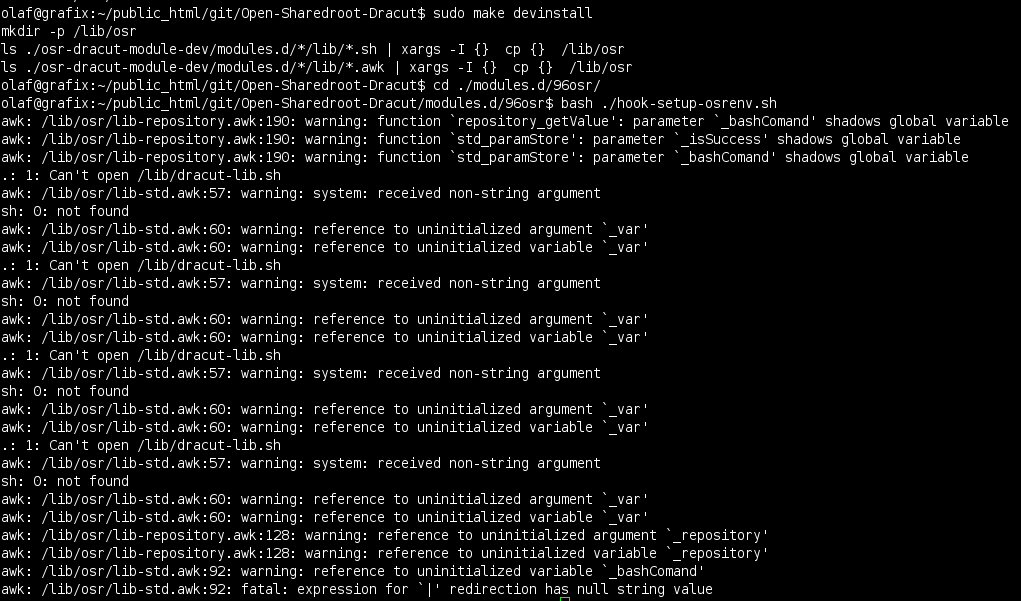
\includegraphics[width=1.0\textwidth]{./awk-lint.png}
 \caption[]{Ausgabe des AWK Lint-Flag}
 \label{pic:lint} 
\end{figure}

\begin{figure}[H]
 \centering
 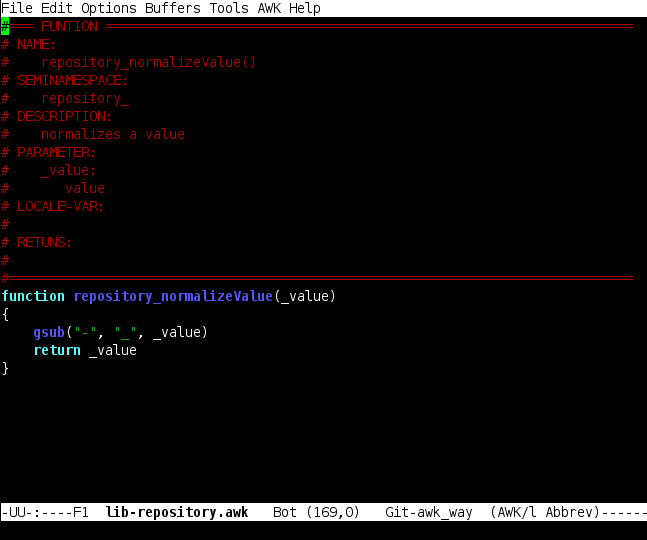
\includegraphics[width=0.75\textwidth]{./awk-emacs.png}
 \caption[]{Syntax highlighting mit Emacs}
 \label{pic:emacs} 
\end{figure}


\begin{figure}[H]
 \centering
 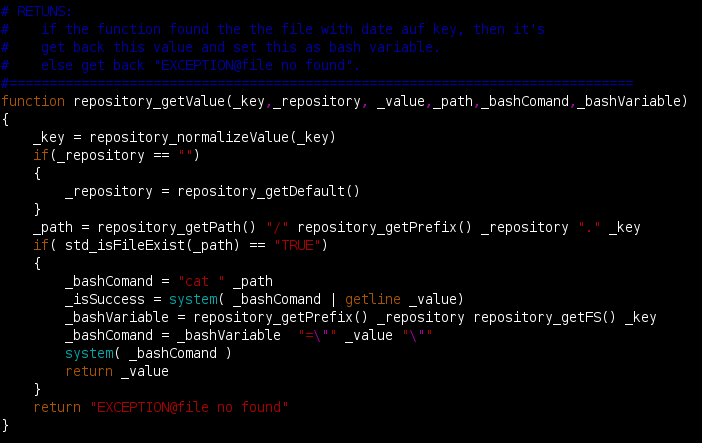
\includegraphics[width=0.75\textwidth]{./awk-vim.png}
 \caption[]{Syntax highlighting mit Vim}
 \label{pic:vim} 
\end{figure}

\begin{figure}[H]
 \centering
 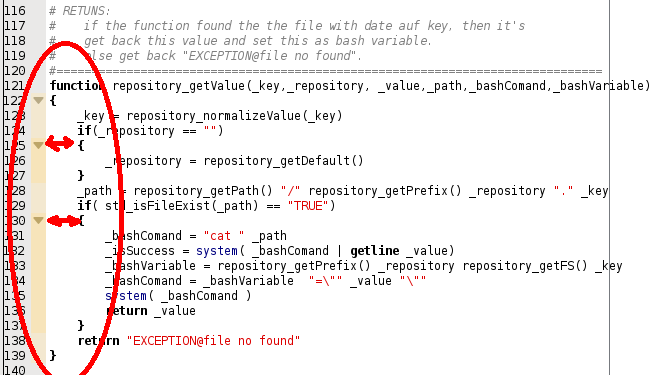
\includegraphics[width=0.75\textwidth]{./awk-kate.png}
 \caption[]{Ausschnitt vom Kate-Editor mit "`Klammer-Falt-Funtktion"'}
 \label{pic:kate}
\end{figure}

\subsubsection{Libs, Namensspace, Kommentare}

AWK hat keinen Namespaces. Stattdessen werden Biblotheken mit Semit-Namespace versehen, getrent mit "`\_"' (Unterstrich). Also z.B.: "`std\_functionsname"'. "`std"' ist in diesem Fall der Namespace. AWK unterscheidet bei Variabeln- und Funktionsnnamen zwischen Groß- und Kleinschreibung. Lange Funktionsnamen können also so gestaltet werden: \texttt{std\_einSehrLangerFunktionsName()}.


Die Dateinamen von Bibliotheken beginnen mit "`lib\_"'. Also z.B. "`lib\_std.awk"' für die Standart-Biblothek. Jede Datei hat zubegin den folgenden Haeder:

\begin{lstlisting}
#!/usr/bin/awk -f
#==============================================================================
# FILE:
#       lib-std.awk
# SEMINAMESPACE:
#       std_
# DESCRIPTION:
#       Standart Lib for com.oonics-dracut-module
# AUTORS:
#       [...]
# COMPANY:
#       ATIX AG
# LIZENZ:
#        [...]
#==============================================================================
\end{lstlisting}
Jede datei hat genau \textbf{EINEN} Namensspace!


\bigskip 


Variablen in AWK sind grundsäzlich global. Nur die Parameter der Funktionen sind lokal. Diese Parameter-Variablen werden \textbf{AUCH} in AWK benutzt, um lokale Variablen ab zu bilden. Lokale Variablen -- wo immer möglich -- globalen vorzuziehen! Es können in AWL-Funktionen mehr Parameter-Variablen definiert werden, als beim Funktionsaufruf verwendet werden. Alle lokalen Variablen haben ein  "`\_"' (Unterstrich) vorangestellt zu haben. Die zwingend zu zu übergebenen Werte werden durch zusätzliche Leerzeichen von den übrigen lokalen Variaben separiert. Die Variablen und Parameter und lokalen Variablen werden in einem Kopf-Kommentar dokumentiert.


\bigskip 
\textbf{Beispiel:}


\begin{lstlisting}
#=== FUNTION ==================================================================
# NAME:
#    osr_paramStore()
# SEMINAMESPACE:
#    std_
# DESCRIPTION:
#    [...]
# PARAMETER:
#    _key: [...]
# LOCALE-VAR:
#    _var: [...]
# RETUNS:
#    [...]
#==============================================================================

std_osr_paramStore(_key, _var)
{
    system(". /lib/dracut-lib.sh; getarg $key 2>/dev/null" | getline _var)
    print _var
}
\end{lstlisting}


AWK unterstützt komplexe Typen. Und zwar ein- und mehrdimensionale Arrays.
Funktionen können leider keine Arrays zurückgeben. Aber Funktionen können Array
übergeben bekommen und manipulieren. Eine objektorientierte
Programmierung ist daher trotzdem möglich und \textbf{sinnvoll}!

\bigskip

\begin{lstlisting}
#!/usr/bin/awk  -f

BEGIN{
    mittagspause()
}

# _peter ist nur in der Funktion mittagspause() sichtbar.
function mittagspause( _peter,_uli,_zombi,_info,_ex)
{
#     _ex[""] = ""
      FactoryFleischesser(_peter)
      FactoryVegetarier(_uli)
      FactoryZombi(_zombi)

      print "vorher: Peter, bauch " _peter["Bauch"]
      print "vorher: Uli, bauch " _uli["Bauch"]

      # goToMcDonalds() ist quasi eine Klasseneigenschaft.
      goToMcDonalds(_peter)
      goToMcDonalds(_uli)

      _info = goToMcDonalds(_zombi)
      if ( ExceptionHandler(_info,_ex) )
      {
          print "Message: "  _ex["message"]
          print "Specification: "  _ex["specification"]
          print "Kein Blud fuer Zombis bei McDonadt!"
      }

      print "nachher: Peter, bauch " _peter["Bauch"]
      print "nachher: Uli, bauch " _uli["Bauch"]
}


# Erstellt ein Objekt der Klasse "Mensch" abgeleitet ist
function FactoryMensch(_mensch)
{
    _mensch["Bauch"] = "leer"
}

# Erstellt ein Objekt der Klasse "Fleischesser" das von Klasse "Mensch" abgeleitet ist
function FactoryFleischesser(_mensch)
{
    FactoryMensch(_mensch)
    _mensch["Typ"] = "Fleischesser"
}

# Erstellt ein Objekt der Klasse "Vegetarier" das von Klasse "Mensch" abgeleitet ist
function FactoryVegetarier(_mensch)
{
    FactoryMensch(_mensch)
    _mensch["Typ"] = "Vegetarier"
}


# Erstellt ein Objekt der Klasse "Zombi" das von Klasse "Mensch" abgeleitet ist
function FactoryZombi(_mensch)
{
    FactoryMensch(_mensch)
    _mensch["Typ"] = "Zombi"
}


# _mensch ist ein uebergebenes Objekt
function goToMcDonalds(_mensch)
{
    if (_mensch["Typ"] == "Fleischesser" )
    {
        _mensch["Bauch"] = "voll"
    }else if (_mensch["Typ"] == "Vegetarier" )
    {
        _mensch["Bauch"] = "leer"
    }else
    {
        return "Exception@TypException@bad typ"
    }
    return ""
}

# Ausname fuer Typen-Fehler
function ExceptionHandler(_info,_ex, _array)
{
    if( index(_info, "Exception@") != 0)
    {
        split(_info, _array, "@")
        _ex["specification"] = _array[2]
        _ex["message"] = _array[3]
        return 1
    }
    return 0
}
\end{lstlisting} 

\bigskip 
Zur Vertiefung des Themas siehe auch: \url{http://de.wikibooks.org/wiki/Awk:_Grundlagen:_Objektorientierte_Programmierung}




\section{Nutzungsbedingungen}

\subsection{Informationen für Weiternutzer}

Du kannst den Inhalt dieser Dokumentation frei weiternutzen. Bitte beachte die
folgenden Leitlinien:

\subsection{Weiterverwendung von Text:}

\begin{itemize}

 \item Namensnennung: Um eine Textseite in irgendeiner Form lizenzkonform
 wiederzuveröffentlichen, musst du die Autoren angeben, entweder
 \begin{itemize}


  \item durch Angabe des Hyperlinks (sofern möglich) oder der URL auf jede
  Seite, die weiterverwandt wird,
  \item durch Angabe des Hyperlinks (sofern möglich) oder der URL auf eine
  alternative, stabile und frei zugängliche Online-Kopie, welche die
  Lizenzbestimmungen einhält und die Autoren auf zu dieser Website adäquater
  Weise nennt,
  \item. oder einer Liste aller Autoren. Jede Autorenliste kann sehr kleine
  oder irrelevante Änderungen übergehen.

  Diese Bestimmungen gelten für Text, der in der Wikimedia-Gemeinschaft
  entstanden ist. Text von außerhalb kann zusätzliche Bedingungen an die
  Namensnennung stellen, welche wir klar aufzuzeigen versuchen werden.
  Beispielsweise kann eine Seite einen Kasten oder eine andere Notiz enthalten,
  dass ihr Inhalt (teilweise) an anderer Stelle erstveröffentlicht wurde.
  Solche Anmerkungen sollten gewöhnlich von Weiternutzern beibehalten werden.

 \end{itemize}
 \item Weitergabe unter gleichen Bedingungen: Wenn du Änderungen an einer Seite
 vornimmst oder Text hinzufügst, muss der neue Text auch unter Creative Commons
 Attribution-Share-Alike License 3.0 oder einer späteren Version stehen.

 \item Änderungen aufzeigen: Veränderungen oder Erweiterungen eines bestehenden
 Werkes müssen auf angemessene Weise angegeben werden. In einem Wiki etwa ist
 eine Notiz in der Versionsgeschichte ausreichend.

 \item Lizenzhinweis: Jede öffentlich zugängliche Kopie oder modifizierte
 Version muss einen Hinweis enthalten, dass das Werk unter der Lizenz CC-BY-SA
 steht, sowie entweder einen Hyperlink beziehungsweise eine URL auf den Text
 der Lizenz oder eine Kopie des Lizenztextes. Eine für diesen Zweck geeignete
 URL ist \url{http://creativecommons.org/licenses/by-sa/3.0/deed.de}.

 \item Weitere Informationen hierzu können dem Lizenzvertrag der
 CC-BY-SA-Lizenz\footnote{\url{http://creativecommons.org/licenses/by-sa/3.0/legalcode}}
 entnommen werden.

\end{itemize}

\subsection{Zusätzliche Textlizenzierung unter der GNU Free Documentation License}

Aus Kompatibilitätsgründen ist der Text, zusätzlich unter den Bedingungen der
\textit{GNU Free Documentation License} verfügbar.


\section{Quellen- und Literaturangaben}
\label{sec:quell}

\begin{itemize}
 \item fedora-Projekt: \url{http://fedoraproject.org/wiki/Dracut}
 \item Projektseite: \url{https://dracut.wiki.kernel.org/}
 \item News: \url{http://git.kernel.org/?p=boot/dracut/dracut.git;a=blob_plain;f=NEWS}
\end{itemize}



\end{document}